\section{The geometry of the SVD}
The geometry of the \svdl \ provides helpful insights into many problems. We will see the a marvelous depiction of the conditioning to a system. We will also see a clear depiction of the singular values as scale factors.

%%
\subsection{The image of a matrix}
A matrix acts on a vector and produces another vector. Looking at this action on unit vectors is helpful. Consider the locus of all possible unit vectors -  the unit circle. The unit vectors are parameterized as
\begin{equation}
  x_{\theta} = \mat{c}{\cos \theta \\ \sin \theta}, \quad \theta\in[0,2\pi).
\end{equation}

Figure \eqref{fig:maps:both} below shows two plots. The unit circle is the plot of $x_{\theta}$ as $\theta$ varies from 0 to 2$\pi$. The ellipse is the vector showing the action of the target matrix on the unit vectors:
\begin{equation}
  y_{\theta} = \A{}x_{\theta} = \mat{r}{\cos \theta + 2\sin \theta\\-\cos \theta + 2\sin \theta}. 
\end{equation}

The ellipse represents the ``image'' of the target matrix; the action of the matrix on the unit vectors. The context here is a graphical representation. Later we will see this word used in the context of vector space. 

\begin{figure}[htbp] %  figure placement: here, top, bottom, or page
   \centering
   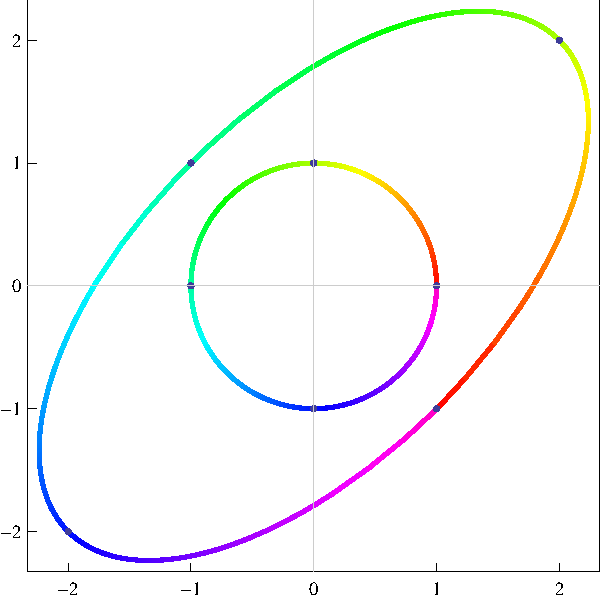
\includegraphics[ width = 2.5in ]{pdf/post_mortemII/dim_22_rank_2_image3} 
   \caption{The mapping action of the matrix in equation \eqref{eq:pmII:A} on all possible unit vectors in $\real{2}$. The coloring of the line is related to the angle. Fiducial marks are shown in increments of $\frac{\pi}{2}$.}
   \label{fig:maps:both}
\end{figure}

The next two plots, in figure \eqref{fig:maps:ev}, separate the curves and adds the eigenvectors. The black arrows are the first eigenvectors and the blue arrows are the second eigenvectors. The unit circle is resolved by the $\X{}$ matrix and the ellipse is resolved by the $\Y{}$ matrix \textit{scaled} by the singular values. This is codified in table \eqref{tab:pmII:blackblue}.

\begin{table}[htdp]
\begin{center}
\boxed{
\begin{tabular}{lrr}
  figure  & blue vector & black vector \\\hline
  circle  & $\X{}_{*,1}$\ \ \ \ \  & $\X{}_{*,2}$\ \ \ \ \  \\
  ellipse & $\sigma_{1} \Y{}_{*,1}$\ \ \ \ \  & $\sigma_{2} \Y{}_{*,2}$\ \ \ \ \ 
\end{tabular}
}
\end{center}
\label{tab:pmII:blackblue}
\caption{The eigenvectors of the domain and codomain and the scaling action of the eigenvectors.}
\end{table}%

This shows the vital relation between the column vectors of the domain and the scaled column vectors of the codomain:
\begin{equation}
  \A{} \X{}_{*,k} = \sigma_{k}\Y{}_{*,k}, \qquad k=1,\rho
  \label{eq:pmII:vital}
\end{equation}
This is of course just a rearrangement of the epitath
$$
\svdax{*}.
$$
The role of the singular values as scale factors is now clear after this demonstration. The blue vectors show the scaling effect of the first singular value; the black vectors the second singular value.

\begin{figure}[htbp] %  figure placement: here, top, bottom, or page
   \centering
   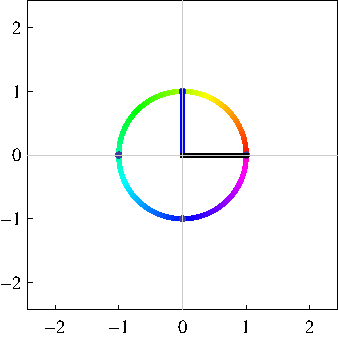
\includegraphics[ width = 2.25in ]{pdf/post_mortemII/circle_ev} \qquad
   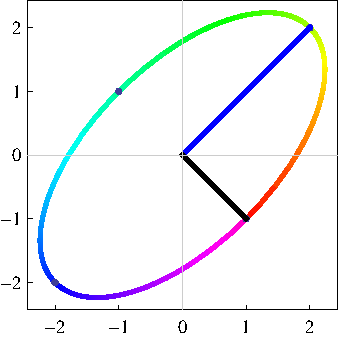
\includegraphics[ width = 2.25in ]{pdf/post_mortemII/ellipse_ev} 
   \caption{The pictorial demonstration of the scaling function of the singular values. The blue vectors show how $\A{} \X{}_{*,1} = \sigma_{k}\Y{}_{*,1}$ and the black vectors show $\A{} \X{}_{*,2} = \sigma_{2}\Y{}_{*,2}$.}
   \label{fig:maps:ev}
\end{figure}

%%
\subsection{The matrix in the simple method}
Look at the map in both directions

%%
\subsubsection{$\A{}x=y$}
\begin{figure}[htbp] %  figure placement: here, top, bottom, or page
   \centering
   \includegraphics[ ]{pdf/post_mortemII/toright} 
   \caption{Examine the mapping action of $\A{}$ from domain to codomain.}
   \label{fig:toright}
\end{figure}

The matrix described in equation \eqref{eq:simple:IamA}.
Recall the first decomposition \eqref{eq:simple:svd}
\begin{equation*}
  \begin{split}
    \svda{T} \\
    \Aexample &= \Yshade \Sigmaexampleb \Xtshade.
  \end{split}
\end{equation*}

Here the rank $\rho=1$ and so there is only one eigenvector to map. The eigenvector $\X{}_{*,1}$ maps to $\sigma_{1}\Y{}_{*,1}$. Since we can't distinctly see the mapping in the 3-dimensional image we show the explicit computation:
\begin{equation}
  \begin{split}
    \A{}\,\X{}_{*,1}\quad &= \quad \sigma_{1}\Y{}_{*,1}, \\
    \Aexample \frac{1}{\sqrt{2}}\mat{r}{1\\-1} \quad & =  \quad \sqrt{6}\frac{1}{\sqrt{3}}\mat{r}{1\\-1\\1}\\
    \frac{2}{\sqrt{2}}\mat{r}{1\\-1\\1}  \quad & =  \quad \sqrt{2}\mat{r}{1\\-1\\1}.
  \end{split}
\end{equation}

Herein lies the problem with the map. The dimension of the image, 1, is less than the dimension of the codomain, 3.

\begin{figure}[htbp] %  figure placement: here, top, bottom, or page
   \centering
   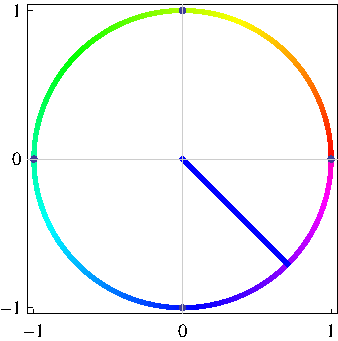
\includegraphics[ width = 1.9in ]{pdf/post_mortemII/a_circle_ev} \qquad
   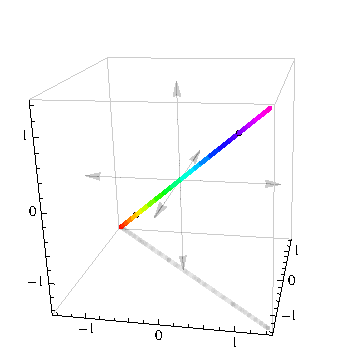
\includegraphics[ ]{pdf/post_mortemII/dim_32_rank_1_image} 
   \caption{The trouble with the matrix $\A{}$ (equation \eqref{eq:simple:IamA}) as a map from domain to codomain. The codomain has dimension 3 yet the image of the target matrix is a line with dimension 1. Because the line is embedded in a $3-$space a point on the line has three coordinates. But along the line there is only one coordinate measuring distance from the origin.}
   \label{fig:toright}
\end{figure}

%%
\subsubsection{$\A{T}y=x$}
\begin{figure}[htbp] %  figure placement: here, top, bottom, or page
   \centering
   \includegraphics[ ]{pdf/post_mortemII/toleft} 
   \caption{Examine the mapping action of the transpose matrix $\A{T}$ from codomain to domain.}
   \label{fig:toright}
\end{figure}
\begin{equation}
  \begin{split}
    \A{T} &= \svdt{T} \\
    \Atexample &= \Xshade \Sigmatexamplea \Ytshade.
  \end{split}
  \label{eq:simple:IamAT}
\end{equation}

\begin{equation}
  \begin{split}
    \A{}\,\X{}_{*,1}\quad &= \quad \sigma_{1}\Y{}_{*,1}, \\
    \Atexample \frac{1}{\sqrt{3}}\mat{r}{1\\-1\\1} \quad & =  \quad \sqrt{6}\frac{1}{\sqrt{2}}\mat{r}{1\\-1}\\
    \frac{3}{\sqrt{3}}\mat{r}{1\\-1}  \quad & =  \quad \sqrt{3}\mat{r}{1\\-1}.
  \end{split}
\end{equation}

\begin{figure}[htbp] %  figure placement: here, top, bottom, or page
   \centering
   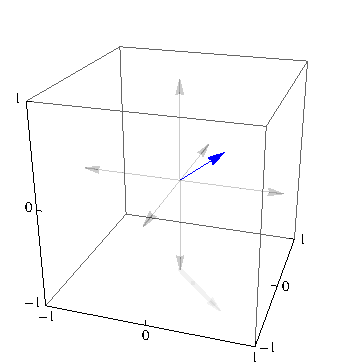
\includegraphics[ ]{pdf/post_mortemII/3_vector}  \qquad
   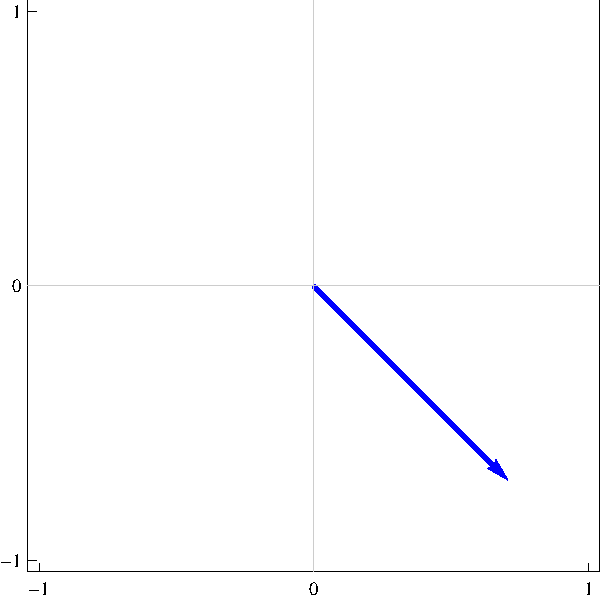
\includegraphics[ width = 1.9in ]{pdf/post_mortemII/430}
   \caption{The trouble with the matrix $\A{T}$ (equation \eqref{eq:simple:IamAT}) as a map from codomain to domain. The codomain has dimension 3 yet the image of the target matrix is a line with dimension 1. Because the line is embedded in a $2-$space a point on the line has two coordinates. But along the line there is only one coordinate measuring distance from the origin.}
   \label{fig:toleft}
\end{figure}

%%
\subsection{The matrix in the general method}
Look at the map in both directions

%%
\subsubsection{Domain $\longrightarrow$ cdomain}
\begin{figure}[htbp] %  figure placement: here, top, bottom, or page
   \centering
   \includegraphics[ ]{pdf/post_mortemII/toright} 
   \caption{Examine the mapping action of $\A{}$ from domain to codomain.}
   \label{fig:toright}
\end{figure}

Start with the first decomposition \eqref{eq:gen:soln}.
\begin{equation}
  \begin{split}
    \A{} &= \Y{}\paren{\sig{}\,\X{T}},\\
     &=
  \frac{1}{\sqrt{2}}
  \mat{rr}{1 & -1\\1 & 1}
  \frac{1}{\sqrt{2}}
  \paren{
  \mat{crc}
  {
  1 & 5  & 2 \\
  1 & -1 & 2
  }}, \\
  &=
  \mat{ccc}
  {
  0 & 3 & 0 \\
  1 & 2 & 2
  }.
  \end{split}
  \label{eq:gen:soln}
\end{equation}

Here the rank $\rho=1$ and so there is only one eigenvector to map. The eigenvector $\X{}_{*,1}$ maps to $\sigma_{1}\Y{}_{*,1}$. Since we can't distinctly see the mapping in the 3-dimensional image we show the explicit computation:
\begin{equation}
  \begin{split}
    \A{}\,\X{}_{*,1}\quad &= \quad \sigma_{1}\Y{}_{*,1}, \\
    \Aexample \frac{1}{\sqrt{2}}\mat{r}{1\\-1} \quad & =  \quad \sqrt{6}\frac{1}{\sqrt{3}}\mat{r}{1\\-1\\1}\\
    \frac{2}{\sqrt{2}}\mat{r}{1\\-1\\1}  \quad & =  \quad \sqrt{2}\mat{r}{1\\-1\\1}.
  \end{split}
\end{equation}

Herein lies the problem with the map. The dimension of the image, 1, is less than the dimension of the codomain, 3.

\begin{figure}[htbp] %  figure placement: here, top, bottom, or page
   \centering
   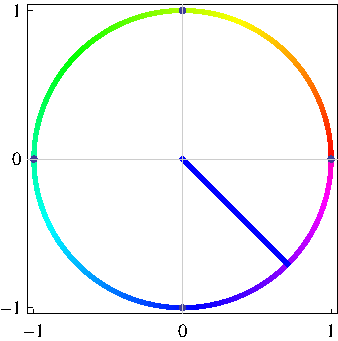
\includegraphics[ width = 1.9in ]{pdf/post_mortemII/a_circle_ev} \qquad
   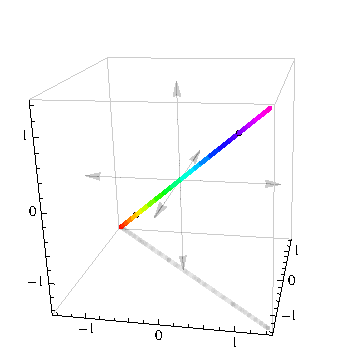
\includegraphics[ ]{pdf/post_mortemII/dim_32_rank_1_image} 
   \caption{The trouble with the matrix $\A{}$ (equation \eqref{eq:simple:IamA}) as a map from domain to codomain. The codomain has dimension 3 yet the image of the target matrix is a line with dimension 1. Because the line is embedded in a $3-$space a point on the line has three coordinates. But along the line there is only one coordinate measuring distance from the origin.}
   \label{fig:toright}
\end{figure}

%%
\subsubsection{$\A{T}y=x$}
\begin{figure}[htbp] %  figure placement: here, top, bottom, or page
   \centering
   \includegraphics[ ]{pdf/post_mortemII/toleft} 
   \caption{Examine the mapping action of the transpose matrix $\A{T}$ from codomain to domain.}
   \label{fig:toright}
\end{figure}
\begin{equation}
  \begin{split}
    \A{T} &= \svdt{T} \\
    \Atexample &= \Xshade \Sigmatexamplea \Ytshade.
  \end{split}
  \label{eq:simple:IamAT}
\end{equation}

\begin{equation}
  \begin{split}
    \A{}\,\X{}_{*,1}\quad &= \quad \sigma_{1}\Y{}_{*,1}, \\
    \Atexample \frac{1}{\sqrt{3}}\mat{r}{1\\-1\\1} \quad & =  \quad \sqrt{6}\,\frac{1}{\sqrt{2}}\mat{r}{1\\-1}\\
    \frac{3}{\sqrt{3}}\mat{r}{1\\-1}  \quad & =  \quad \sqrt{3}\mat{r}{1\\-1}.
  \end{split}
\end{equation}

\begin{figure}[htbp] %  figure placement: here, top, bottom, or page
   \centering
   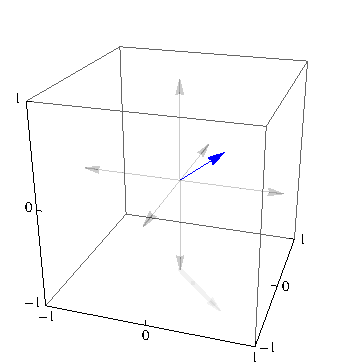
\includegraphics[ ]{pdf/post_mortemII/3_vector}  \qquad
   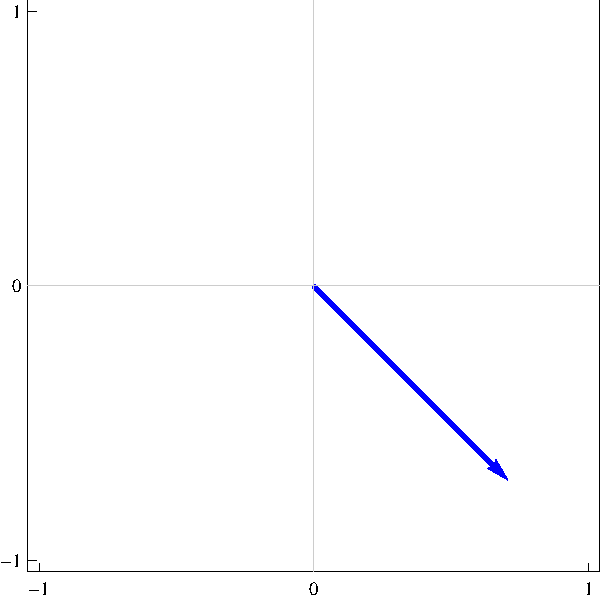
\includegraphics[ width = 1.9in ]{pdf/post_mortemII/430}
   \caption{The trouble with the matrix $\A{T}$ (equation \eqref{eq:simple:IamAT}) as a map from codomain to domain. The codomain has dimension 3 yet the image of the target matrix is a line with dimension 1. Because the line is embedded in a $2-$space a point on the line has two coordinates. But along the line there is only one coordinate measuring distance from the origin.}
   \label{fig:toleft}
\end{figure}


\endinput